\documentclass[bigger]{beamer}

% packages
\usepackage[greek, english]{babel}
\usepackage{lipsum}
\usepackage{graphicx}
\usepackage{subcaption}
\usepackage{fancybox}
\usepackage[export]{adjustbox}
\usepackage{braket}
\usepackage{hyperref}

% colors
\definecolor{purple}{rgb}{0.54, 0.17, 0.89}

% hyperlink coloring
\hypersetup{
    colorlinks = true,
    linkcolor  = purple,
    filecolor  = purple,      
    urlcolor   = purple,
}

% commands
\newcommand{\blank}[1]{\hspace*{#1}}
\newcommand{\mysp}{\blank{0.3cm}}
\newcommand{\lt}[1]{\latintext #1\greektext}
\newcommand{\gt}[1]{\greektext #1\latintext}
\newcommand{\blt}[1]{\lt{\textbf{#1}}}
\newcommand{\tb}[1]{\textbf{#1}}
\newcommand{\ti}[1]{\textit{#1}}
\newcommand{\lorem}{\lt{\lipsum[1]}}

% beamer customization
\usebackgroundtemplate{
\includegraphics[width=\paperwidth, height=\paperheight]{images/template.png}}
\setbeamertemplate{frametitle}{\insertframetitle\par\vspace{0.5em}}
\setbeamercolor{normal text}{fg=white}\usebeamercolor*{normal text}
\setbeamercolor{frametitle}{fg=white}\usebeamercolor*{normal text}
\setbeamersize{text margin left=0.5cm}

% Customize the title page template to align the title to the left
\setbeamertemplate{title page}{
  \begin{flushleft}
    \usebeamerfont{title}\inserttitle\par
    \usebeamerfont{subtitle}\insertsubtitle\par
    \bigskip
    \usebeamerfont{author}\insertauthor\par
    \bigskip
    \usebeamerfont{date}\insertdate\par
  \end{flushleft}
}

% Redefine the frametitle template to align it to the left
\makeatletter
\setbeamertemplate{frametitle}{%
  \nointerlineskip%
  \usebeamerfont{frametitle}%
  \begin{beamercolorbox}[sep=0.3cm,ht=1.8em,wd=\paperwidth]{frametitle}%
    \vbox{}\vskip-2ex%
    \strut\insertframetitle\strut
    \vskip-0.8ex%
  \end{beamercolorbox}%
}
\makeatother

\raggedright

\title{\tb{Color-coding Similarity in\\ Sequence Alignment}}
\author{Asimakis Kydros \\ 3881 \\ \texttt{asimakis@csd.auth.gr}}
\date{\today}

\begin{document}

\frame{\titlepage}

\begin{frame}{\tb{Purpose of Color Schemes}}
    \footnotesize
    
    In sequence alignment, it's useful to color\\
    the amino acids in a way that predicts\\
    their similarity, so we can check\\
    with a glance the estimated alignment.

    \hfill

    Typically, this is done manually, by\\ 
    experienced scientists, using colors according\\
    to pre-determined physical properties,\\
    such as charge.

    \hfill

    This isn't perfect multiple-fold, as two amino acids\\
    having a similar property doesn't always ensure that\\
    their alignment will be optimal in the given context.\\
    Also, we would like an automated solution for every\\
    situation.
    
\end{frame}

\begin{frame}{\tb{Substitution Matrix Schema}}
    \footnotesize

    A better way to do this is to use the given\\
    substitution matrix and a chosen color space,\\
    and define through them a scoring function.\\
    Then, optimize that to approximate the optimal.

    \hfill

    Given the substitution matrix $M$, define
    \newline\\
    {
        \scriptsize
        \mysp $
        D' \ni \Biggl( D'_{ij} = \begin{cases}
                     \frac{M_{ii} - M_{ij} + M_{jj} - M_{ji}}{2}, &j \leq i\\
                                                               0, &j > i
                  \end{cases} \Biggr)
        \xrightarrow{\text{scaled to average 1}} D
        $
    }
    \newline\\
    and the chosen color space \ti{CIE L*a*b*}, define
    \newline\\
    {
        \scriptsize
        \mysp $
        C \ni \Biggl( C_{ij} \approx \sqrt{(L^*_i - L^*_j)^2 + (a^*_i - a^*_j)^2 + (b^*_i - b^*_j)^2} \Biggr)
        $
    }
    \newline\\
    These are triangular matrices that define\\
    the pairwise distance and color variance respectively.
    
\end{frame}

\begin{frame}{\tb{Substitution Matrix Schema}}
    \footnotesize
    
    We can now define the score function
    \newline\\
    {
        \scriptsize
        \mysp $S_T = S_H + S_C$\\
        \hfill

        \text{where}\\
        \mysp $S_H = \sum_{ij}(f_sC_{ij} - D_{ij})^2$\\
        \mysp $S_C = \frac{f_C}{\braket{C}}$\\
        \mysp $f_s = \frac{\braket{D}}{\braket{C}}$\\
        \mysp $\braket{\cdot} \text{ the arithmetic mean}$\\
        \mysp $f_C \text{ a given hyperparameter}$
    }
    \newline\\
    which essentially defines the total square error\\
    of the scaled color variance to distance for\\
    each pair, $S_H$, biased by the contrast enabler $S_C$.

    \hfill

    This function describes a (generally) non-convex problem\\
    that adequately combines the data into\\
    the desired effect: coloring based on distance.\\
    It can be optimized with Simulated Annealing.
    
\end{frame}

\begin{frame}{\tb{Results}}
    \footnotesize
    
    \begin{columns}[T, onlytextwidth]
        \begin{column}{0.45\textwidth}
            The figure grid compares this algorithm's outputs (A, B, C and D) to some given
            color schema made manually.

            \hfill

            We can see that the approaches agree on color similarity, but differ on color dissimilarity; the palette on A and B is more gradient and nuanced than the one on 'Typical', which has very sharp changes.

            \hfill

            The versatility of the method is also emphasized; Figure C is adapted to red-green colorblindness by removing green as an option. Figure D uses a different alphabet altogether, the protein blocks.
        \end{column}
        
        \begin{column}{0.55\textwidth}
            \begin{figure}
                \begin{subfigure}[t]{.4\linewidth}
                    \tb{A} - {\scriptsize \ti{BLOSUM62}}
                    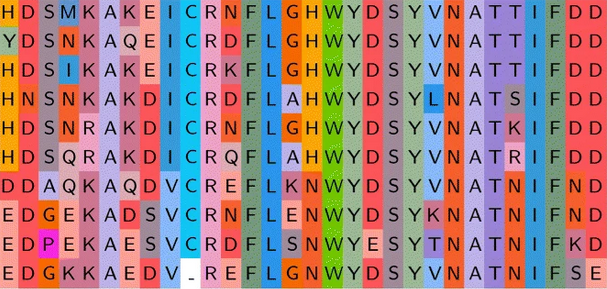
\includegraphics[scale=0.2, valign=t, frame]{images/A.png}
                \end{subfigure}\hfill
                \begin{subfigure}[t]{.4\linewidth}
                    \tb{B} - {\scriptsize \ti{PAM250}}
                    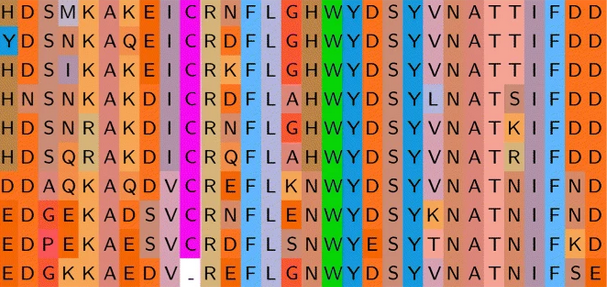
\includegraphics[scale=0.2, valign=t, frame]{images/B.png}
                \end{subfigure}
    
                \medskip

                \begin{subfigure}[t]{.4\linewidth}
                    \tb{Typical}
                    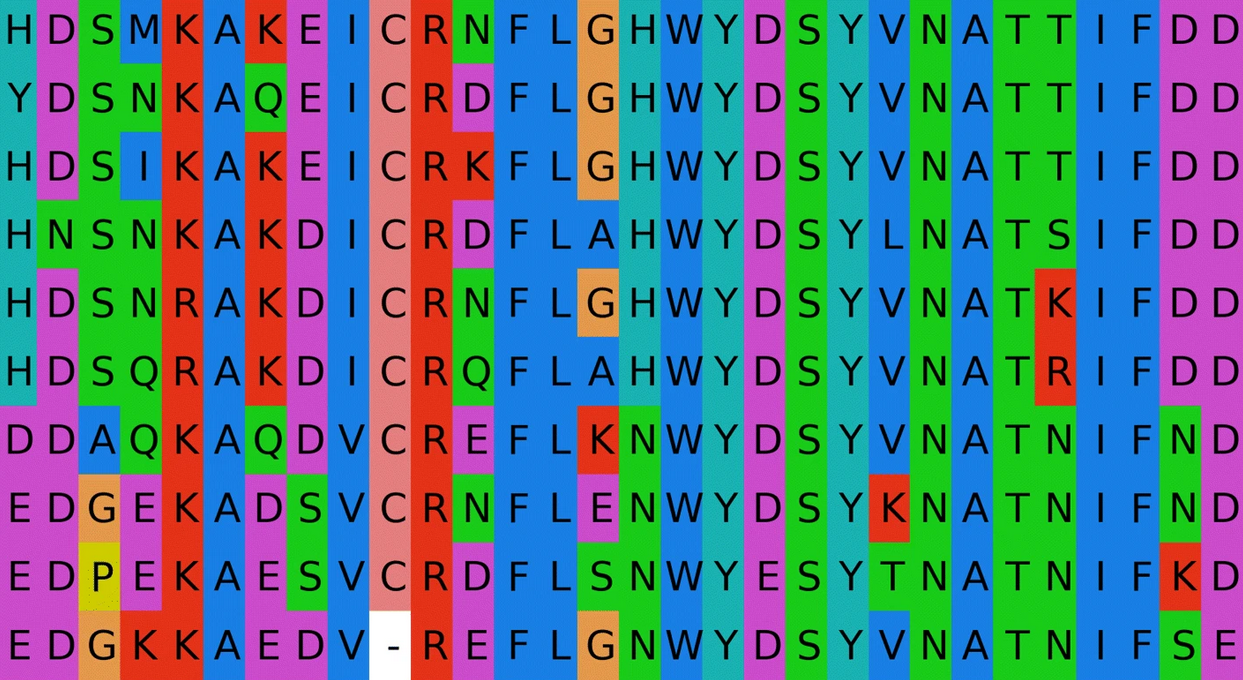
\includegraphics[scale=0.1, valign=t, frame]{images/typical.png}
                \end{subfigure}

                \medskip
                
                \begin{subfigure}[t]{.4\linewidth}
                    \tb{C}
                    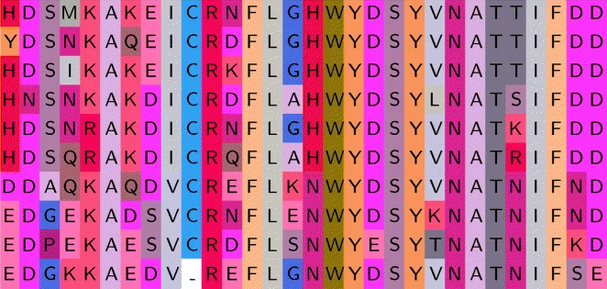
\includegraphics[scale=0.2, valign=t, frame]{images/C.png}
                \end{subfigure}\hfill
                \begin{subfigure}[t]{.4\linewidth}
                    \tb{D}
                    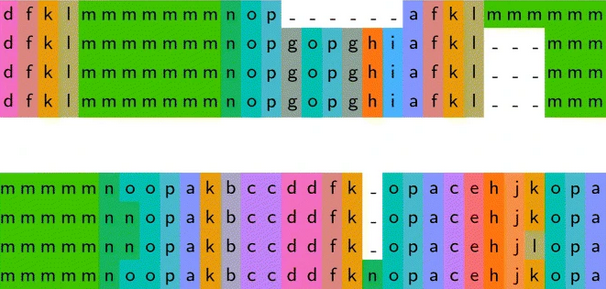
\includegraphics[scale=0.2, valign=t, frame]{images/D.png}
                \end{subfigure}
            \end{figure}
        \end{column}
    \end{columns}
\end{frame}

\begin{frame}{\tb{Conclusions}}
    \footnotesize

    This tool does a terrific job projecting\\
    the relationships between amino acids\\
    anchored on molecular evolution rather\\
    than anything else, thus tying them to\\
    the problem of sequence alignment.

    \hfill
    
    It enables the automatic and independent\\
    calculation of sequence alignment heat maps,\\
    without the need for research of physical\\
    characteristics and unnecessary modeling.

    \hfill

    Its generic definition also allows it to be applied\\
    to fields other than bioscience, be it for understanding\\
    exotic alphabets, cryptographic concepts and much more.
    
\end{frame}

\begin{frame}{\tb{References}}
    \footnotesize
    Principal paper:
    \newline\\
    $\circ$ Kunzmann, P.; Mayer, B.E.;\\ \mysp Hamacher, K. (2020)\\
    \href{https://bmcbioinformatics.biomedcentral.com/articles/10.1186/s12859-020-3526-6}
    {\mysp \ti{"Substitution matrix based color schemes\\ \mysp for sequence alignment visualization"}}
    \newline\\

    Secondary sources:
    \newline\\
    $\circ$ The course's slides and notes.\\
    $\circ$ Wikipedia
    \href{https://en.wikipedia.org/wiki/Multiple_sequence_alignment}
    {\mysp \ti{"Multiple sequence alignment"}}
    
\end{frame}

\end{document}